\section{Lightweight Encryption/Authentication }


Authenticate encryption is a method of providing confidentiality and message integrity at the same time with one call of operation. While confidentiality comes from the generated cypher, authentication or integrity comes from the tag generated during encryption. Upon receiving, the receiver can decrypt the cypher to get the plan message as well as check the tag is the same in order to check neither the message nor the cypher has been modified upon transmission.

\subsection{AES-GCM}


\subsection{ASCON}

ASCON is an authenticate encryption algorithm designed and developed by A, B, C and at University. Though it has been under the curtain for years, it become very popular after it wins CASEAR NIST computation. The authors claim the main goal of the algorithm is to provide simplicity, online, security, side-channel robustness, single-pass and lightweight cipher for the resource-constrained device. It is is also a well-performing algorithm for short messages \cite{dobraunigAsconV1Lightweight2021} like for applications to collect environment and operating condition in industry 4.0

The algorithm can also be used on high-performin machines to provide encryption and decryption for  time-critical applications. It can provide 128-bit key security \cite{dobraunigAsconV1Lightweight2021}, surpassing the currently accepted 80-bit security standard.


\begin{figure}[H]
    \centering
    \caption{ASCON encryption }
    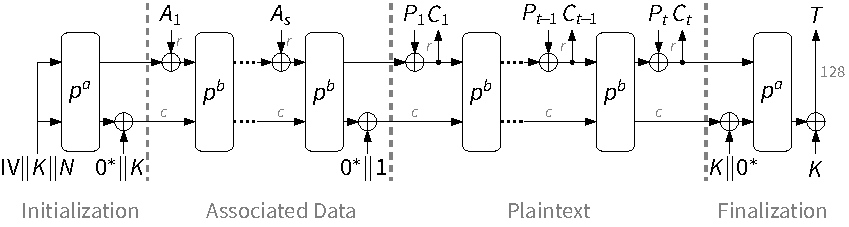
\includegraphics{images/fp/aead_encrypt.pdf}
    \label{fig:ascon-enc}
\end{figure}

The encryption and decryption process of ASCON is split into 4 main phases is depicted in Figure \ref{fig:ascon-enc, fig:ascon-dec}. These are initialization, associated data processing, plain text/cipher text processing (depending on whether it is in encryption or decryption mod) and finalization. 



\begin{figure}[H]
    \centering
    \caption{ASCON decryption}
    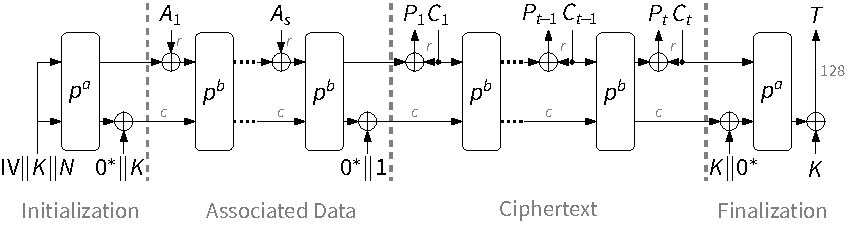
\includegraphics{images/fp/aead_decrypt.pdf}
    \label{fig:ascon-dec}
\end{figure}
